\documentclass[]{plantilla-material-v1}

\def\colegio{Colegio Latinoamericano de Integración}
\def\titulo{Guía}
\def\subtitulo{Proporciones}

\begin{document}

\section{¿Qué es una proporción directa?}

\begin{importante}
  Es cuando dos cantidades crecen o disminuyen juntas, cuando una se multiplica por 
  un número la otra queda multiplicada por el mismo número, o al dividir una 
  de ellas la otra cantidad queda dividida por el mismo número. 
\end{importante}

Determine si los valores relacionados están en proporción directa.

\begin{ejercicios}[after-item-skip=5pt](1)
  \ejercicio La cantidad de personas que pagan su entrada a un evento y la
  ganancia obtenida.
  \ejercicio La cantidad de libros que contiene una caja y el peso de esta.
  \ejercicio La edad del hermano mayor de Jorge, que tiene 5 años más que él.
  \ejercicio La cantidad de máquinas que realizan un trabajo y el tiempo que tardarán
  en terminarlo.
  \ejercicio La cantidad de minutos de una llamada y el valor que se paga.
\end{ejercicios}

\section{Proporción directa como tabla}
\begin{center}
  \vspace{5pt}
  \begin{tblr}{colspec={rccl},cells={mode=math},vline{2-4}={solid},hlines={2-3}{solid},
    column{1}={rightsep+=15pt},column{4}={leftsep+=15pt},cell{1}{2,3}={black!10}}
                    &  x   &  y   &           \\
      1\div4=0,25   &  1   &  4   &  4\div1=4 \\
      2\div8=0,25   &  2   &  8   &  8\div4=4 \\
      3\div12=0,25   &  3   &  12   &  12\div3=4 \\
  \end{tblr}
  \vspace{5pt}
\end{center}

\begin{importante}
  Se mantiene la división entre los valores, a $4$ o $0,25$
  se les llama constante de proporcionalidad.  
\end{importante}

Analiza las tablas y determina si las variables son directamente proporcionales.

\begin{ejercicios}[resume,after-item-skip=15pt](2)
  \ejercicio \begin{tblr}{colspec={cc},row{1}={black!10},vlines,hlines,cells={mode=math}}
    x & y \\
    1 & 3 \\
    2 & 6 \\
    3 & 9 \\
  \end{tblr}
  \ejercicio \begin{tblr}{colspec={cc},row{1}={black!10},vlines,hlines,cells={mode=math}}
    a & b \\
    6 & 8 \\
    12 & 4 \\
    18 & 2 \\
  \end{tblr}
  \ejercicio \begin{tblr}{colspec={cc},row{1}={black!10},vlines,hlines,cells={mode=math}}
    c & d \\
    6 & 1.5 \\
    4 & 1 \\
    10 & 2.5 \\
  \end{tblr}
  \ejercicio \begin{tblr}{colspec={cc},row{1}={black!10},vlines,hlines,cells={mode=math}}
    e & f \\
    7 & 49 \\
    5 & 35 \\
    3 & 21 \\
  \end{tblr}
\end{ejercicios}

\section{Proporción directa como ecuación}

\def\mejemplo{\begin{tblr}{colspec={cc},row{1}={black!10},vlines,hlines,cells={mode=math}}
  a & b \\
  3 & 6 \\
  15 & x \\
\end{tblr}}

\begin{center}
  \figuraTriple{\mejemplo}{$\iff$}{$\dfrac{3}{6}=\dfrac{15}{x}$}[5pt]
\end{center}

Se puede encontrar $x$ despejando, es decir,
\begin{equation*}
  x = \dfrac{15\cdot 6}{3} = 30.
\end{equation*}

Determinar el valor del elemento que falta en cada una de las siguientes proporciones
\begin{ejercicios}[resume,after-item-skip=10pt](3)
  \ejercicio $\dfrac{3}{4}=\dfrac{x}{8}$ 
  \ejercicio $\dfrac{2}{n}=\dfrac{8}{32}$ 
  \ejercicio $\dfrac{4}{5}=\dfrac{12}{m}$ 
  \ejercicio $\dfrac{a}{5}=\dfrac{6}{15}$ 
  \ejercicio $\dfrac{20}{x}=\dfrac{6}{15}$ 

  \ejercicio $\dfrac{7}{14}=\dfrac{y}{10}$ 
  \ejercicio $\dfrac{x}{4}=\dfrac{6}{2}$ 
  \ejercicio $\dfrac{2}{3}=\dfrac{12}{n}$ 
  \ejercicio $\dfrac{7}{8}=\dfrac{56}{p}$ 
  \ejercicio $\dfrac{x}{8}=\dfrac{9}{12}$ 

  \ejercicio $\dfrac{3}{7}=\dfrac{z}{28}$ 
  \ejercicio $\dfrac{y}{5}=\dfrac{8}{20}$ 
  \ejercicio $\dfrac{3}{9}=\dfrac{x}{27}$ 
  \ejercicio $\dfrac{x}{100}=\dfrac{150}{75}$ 
  \ejercicio $\dfrac{15}{70}=\dfrac{30}{x}$ 

  \ejercicio $\dfrac{5}{m}=\dfrac{15}{9}$ 
  \ejercicio $\dfrac{3}{5}=\dfrac{12}{m}$ 
  \ejercicio $\dfrac{90}{x}=\dfrac{15}{85}$ 
  \ejercicio $\dfrac{8}{a}=\dfrac{16}{12}$ 
  \ejercicio $\dfrac{4}{12}=\dfrac{x}{3}$ 
\end{ejercicios}

\section{Proporción directa como gráfico}

\begin{importante}
  Los puntos de la recta forman una proporción directa. Ejemplo: La tarifa que cobra 
una compañía de teléfonos según los minutos que se habla.
\end{importante}

% \begin{tcbraster}[enhanced,raster columns=3,raster width=\linewidth,raster column skip=3pt,raster force size=false]  
%     \begin{tcolorbox}[blankest]
%       \begin{tikzpicture}[line width=1pt,x=0.5cm,y=0.7cm]
%         \draw[->] (0,0) node[below left] {0} -- (5.5,0) node[midway,yshift=-25pt] {Minuto ($m$)};
%         \draw[->] (0,0) -- (0,5.5) node[midway,sloped,yshift=+25pt] {Valor ($v$)};
%         \foreach \x in {1,...,5} {
%           \draw (\x,-0.2) node[below] {$\x$} -- (\x,0.2);
%         }
%         \foreach \y in {1,...,5} {
%           \pgfmathsetmacro{\result}{int(10*\y)}
%           \draw (-0.2,\y) node[left]{$\result$} -- (0.2,\y);
%         }
%         \draw[->] (0,0) -- (1,2) node[shape=circle,fill,inner sep=2pt] (A) {} -- (2,4) node[shape=circle,fill,inner sep=2pt] (B) {} -- ([turn]0:15pt);
%         \draw[dashed] (0,0 -| A) -- (A) -- (0,0 |- A);
%         \draw[dashed] (0,0 -| B) -- (B) -- (0,0 |- B);
%       \end{tikzpicture}
%     \end{tcolorbox}
%     \begin{tcolorbox}[blankest]
%       \begin{equation*}
%         \iff
%       \end{equation*}
%     \end{tcolorbox}
%     \begin{tcolorbox}[blankest]
%       \begin{tblr}{colspec={cc},row{1}={black!10},vlines,hlines,cells={mode=math}}
%         m & v \\
%         1 & 20 \\
%         2 & 40 \\
%       \end{tblr}
%     \end{tcolorbox}
% \end{tcbraster}

\def\figGrap{
  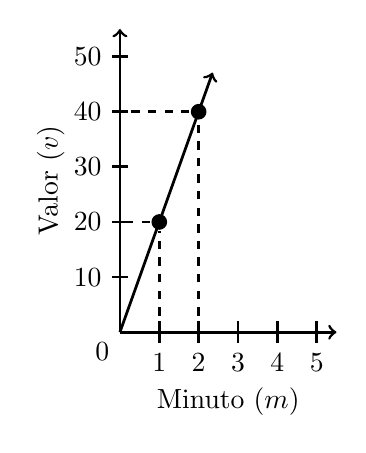
\begin{tikzpicture}[line width=1pt,x=0.5cm,y=0.7cm]
    \draw[->] (0,0) node[below left] {0} -- (5.5,0) node[midway,yshift=-25pt] {Minuto ($m$)};
    \draw[->] (0,0) -- (0,5.5) node[midway,sloped,yshift=+25pt] {Valor ($v$)};
    \foreach \x in {1,...,5} {
      \draw (\x,-0.2) node[below] {$\x$} -- (\x,0.2);
    }
    \foreach \y in {1,...,5} {
      \pgfmathsetmacro{\result}{int(10*\y)}
      \draw (-0.2,\y) node[left]{$\result$} -- (0.2,\y);
    }
    \draw[->] (0,0) -- (1,2) node[shape=circle,fill,inner sep=2pt] (A) {} -- (2,4) node[shape=circle,fill,inner sep=2pt] (B) {} -- ([turn]0:15pt);
    \draw[dashed] (0,0 -| A) -- (A) -- (0,0 |- A);
    \draw[dashed] (0,0 -| B) -- (B) -- (0,0 |- B);
  \end{tikzpicture}
}
\def\figTab{
  \begin{tblr}{colspec={cc},row{1}={black!10},vlines,hlines,cells={mode=math}}
    m & v \\
    1 & 20 \\
    2 & 40 \\
  \end{tblr}
}

\figuraTriple{\figGrap}{$\iff$}{\figTab}

\begin{ejercicios}[resume](1)
  \ejercicio 
  La tabla corresponde a las tarifas cobradas por dos estacionamientos.

  \vspace*{10pt}
  \begin{tblr}{colspec={cccc},row{1}={black!10},vlines,hlines, cell{1}{1,3}={r=1,c=2}{c}}
    Estacionamiento A & 1-2 & Estacionamiento B & 1-4 \\
    N° Horas & Cobro & N° Horas & Cobro \\
    1        & \$630         & 1        & \$830          \\
    2        & \$1260         & 2        & \$1430          \\
    3        & \$1890        & 3        & \$2030        \\
    4        & \$2520        & 4        & \$2630         \\
    5        & \$3150        & 5        & \$3230         \\
  \end{tblr}
  \vspace{5pt}
  \begin{preguntas}
    \pregunta ¿En qué estacionamiento la tarifa corresponde a una proporción directa? Justifica.
    \pregunta ¿Qué estacionamiento es más económico por 5 horas? Explica.
    \pregunta ¿Qué estacionamiento es más económico al permanecer 7 horas? ¿Por qué?
    \pregunta Confecciona un gráfico para representar las tarifas de ambos estacionamientos.
  \end{preguntas}
\end{ejercicios}

Analiza los gráficos y determina el valor desconocido de las siguientes variables 
que están en proporción directa.
\begin{ejercicios}[resume](2)
  \ejercicio 
  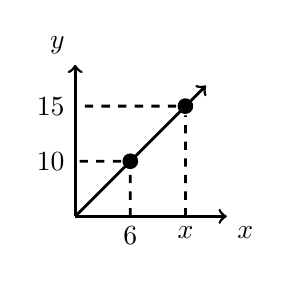
\begin{tikzpicture}[line width=1pt,scale=0.35,baseline=(current bounding box.north)]
    \draw[->] (0,0) -- (5.5,0) node[pos=1,below right] {$x$};
    \draw[->] (0,0) -- (0,5.5) node[pos=1,above left] {$y$};
    \draw[->] (0,0) -- (2,2) node[shape=circle,fill,inner sep=2pt] (A) {} -- (4,4) node[shape=circle,fill,inner sep=2pt] (B) {} -- ([turn]0:30pt);
    \draw[dashed] (0,0 -| A) node [below]{6} -- (A) -- (0,0 |- A) node [left]{10};
    \draw[dashed] (0,0 -| B) node[below]{$x$} -- (B) -- (0,0 |- B) node [left]{15};
  \end{tikzpicture}
  \ejercicio 
  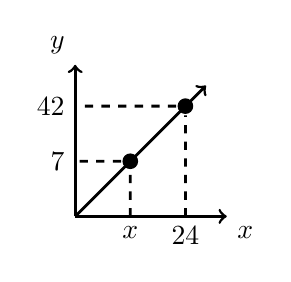
\begin{tikzpicture}[line width=1pt,scale=0.35,baseline=(current bounding box.north)]
    \draw[->] (0,0) -- (5.5,0) node[pos=1,below right] {$x$};
    \draw[->] (0,0) -- (0,5.5) node[pos=1,above left] {$y$};
    \draw[->] (0,0) -- (2,2) node[shape=circle,fill,inner sep=2pt] (A) {} -- (4,4) node[shape=circle,fill,inner sep=2pt] (B) {} -- ([turn]0:30pt);
    \draw[dashed] (0,0 -| A) node [below]{$x$} -- (A) -- (0,0 |- A) node [left]{7};
    \draw[dashed] (0,0 -| B) node[below]{24} -- (B) -- (0,0 |- B) node [left]{42};
  \end{tikzpicture}
  \ejercicio 
  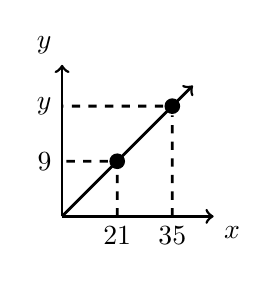
\begin{tikzpicture}[line width=1pt,scale=0.35,baseline=(current bounding box.north)]
    \draw[->] (0,0) -- (5.5,0) node[pos=1,below right] {$x$};
    \draw[->] (0,0) -- (0,5.5) node[pos=1,above left] {$y$};
    \draw[->] (0,0) -- (2,2) node[shape=circle,fill,inner sep=2pt] (A) {} -- (4,4) node[shape=circle,fill,inner sep=2pt] (B) {} -- ([turn]0:30pt);
    \draw[dashed] (0,0 -| A) node [below]{21} -- (A) -- (0,0 |- A) node [left]{9};
    \draw[dashed] (0,0 -| B) node[below]{35} -- (B) -- (0,0 |- B) node [left]{$y$};
  \end{tikzpicture}
  \ejercicio 
  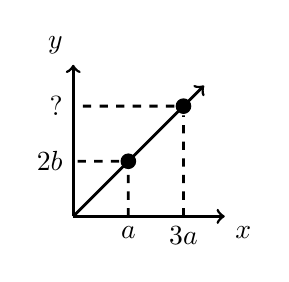
\begin{tikzpicture}[line width=1pt,scale=0.35,baseline=(current bounding box.north)]
    \draw[->] (0,0) -- (5.5,0) node[pos=1,below right] {$x$};
    \draw[->] (0,0) -- (0,5.5) node[pos=1,above left] {$y$};
    \draw[->] (0,0) -- (2,2) node[shape=circle,fill,inner sep=2pt] (A) {} -- (4,4) node[shape=circle,fill,inner sep=2pt] (B) {} -- ([turn]0:30pt);
    \draw[dashed] (0,0 -| A) node [below]{$a$} -- (A) -- (0,0 |- A) node [left]{$2b$};
    \draw[dashed] (0,0 -| B) node[below]{$3a$} -- (B) -- (0,0 |- B) node [left]{$?$};
  \end{tikzpicture}
\end{ejercicios}

\section{¿Qué es una proporción inversa?}

\begin{importante}
  Es cuando dos cantidades se mueven en direcciones opuestas, cuando una crece 
  y es multiplicada por una cantidad la otra disminuye y es dividida por la misma cantidad.  
\end{importante}

Determina si las magnitudes en las siguientes situaciones son inversamente proporcionales.

\begin{ejercicios}[resume,after-item-skip=5pt](1)
  \ejercicio La cantidad de desagües de un depósito y el tiempo que se demora en vaciarlo.
  \ejercicio La cantidad de maquinarias en una cadena de producción y el tiempo que se demoran
  en elaborar un producto.
  \ejercicio La cantidad de comida que se debe comprar para una familia y la cantidad 
  de integrantes de esta.
  \ejercicio La velocidad a la que circula un automóvil y el tiempo que se demora en llegar
  a destino.
  \ejercicio El ancho de un rectángulo y el largo del mismo para que se conserve su área.
\end{ejercicios}

\section{Proporción inversa como tabla}

\begin{center}
  \begin{tblr}{colspec={ccc},row{1}={black!10},vlines,hlines,cells={valign=m}}
    x & y & {Constante de\\proporcionalidad} \\
    1 & 60 & $1\cdot 60=60$ \\
    2 & 30 & $2\cdot 30=60$ \\
    3 & 20 & $3\cdot 20=60$ \\
    4 & 15 & $4\cdot 15=60$ \\
    5 & 12 & $5\cdot 12=60$ \\
  \end{tblr}
\end{center}

\begin{importante}
  Se mantiene la multiplicación entre ambos valores. En este caso 60 es la constante de
proporcionalidad.
\end{importante}
Determina si las siguientes relaciones corresponden a una 
proporcionalidad inversa.

\begin{ejercicios}[resume,after-item-skip=10pt](1)
  \ejercicio 
    \begin{tblr}{colspec={ccccc},column{1}={black!10},vlines,hlines,cells={valign=m}}
      $t$ & 2 & 3 & 4 & 5 \\
      $u$ & 18 & 12 & 9 & 7,2 \\
    \end{tblr}
  \ejercicio 
    \begin{tblr}{colspec={ccccc},column{1}={black!10},vlines,hlines,cells={valign=m}}
      $p$ & 90 & 92 & 94 & 96 \\
      $q$ & 4 & 6 & 8 & 10 \\
    \end{tblr}
  \ejercicio 
    \begin{tblr}{colspec={ccccc},column{1}={black!10},vlines,hlines,cells={valign=m}}
      $r$ & 22.5 & 20 & 15 & 10 \\
      $s$ & 2 & 2,5 & 3 & 4,5 \\
    \end{tblr}
  \ejercicio 
    \begin{tblr}{colspec={ccccc},column{1}={black!10},vlines,hlines,cells={valign=m}}
      $w$ & 50 & 40 & 30 & 20 \\
      $z$ & 10 & 8 & 6 & 5 \\
    \end{tblr}
\end{ejercicios}

\section{Proporción inversa como gráfico}
\begin{importante}
  Los puntos de una proporción inversa forman una curva que se abre hacia los ejes sin
tocarlos. 
\end{importante}
El siguiente ejemplo muestra la relación que hay entre una tabla de valores y
su gráfica para una proporción inversa.
\begin{center}
  \begin{tikzpicture}[line width=1pt,scale=0.7]
    \def\tabla{
      \begin{tblr}{colspec={cccc},column{1}={black!10},vlines,hlines,cells={valign=m}}
        $y$ & 4 & 2 & 1  \\
        $x$ & 1 & 2 & 4  \\
      \end{tblr}
    }
    \draw[->] (0,0) node[below left] {0} -- (5.5,0) node[pos=1,below right] {$x$};
    \draw[->] (0,0) -- (0,5.5) node[above left] {$y$};
    \foreach \x in {1,...,5} {
      \draw (\x,-0.2) node[below] {$\x$} -- (\x,0.2);
    }
    \foreach \y in {1,...,5} {
      \draw (-0.2,\y) node[left]{$\y$} -- (0.2,\y);
    }
    %\draw [] plot[smooth, tension=1] coordinates {(1,4) (2,2) (4,1)};
    \draw[smooth,domain=0.8:5] plot (\x,4/\x);
    \draw[dashed] (0,0 -| 1,4) -- (1,4) node[shape=circle,fill,inner sep=2pt] {} -- (0,0 |- 1,4);
    \draw[dashed] (0,0 -| 2,2) -- (2,2) node[shape=circle,fill,inner sep=2pt] {} -- (0,0 |- 2,2);
    \draw[dashed] (0,0 -| 4,1) -- (4,1) node[shape=circle,fill,inner sep=2pt] {} -- (0,0 |- 4,1);
    \node[anchor=south west] at (current bounding box.center) {\tabla};
  \end{tikzpicture}  
\end{center}


\begin{ejercicios}(1)
  \ejercicio Completa y grafica la información de la tabla.
  \begin{center}
    \vspace{10pt}
    \begin{tblr}{colspec={cc},row{1}={black!10},vlines,hlines,cells={valign=m}}
      \SetCell[r=1,c=2]{c} Velocidad del automóvil & \\
      Velocidad ($v$) & Horas ($h$)  \\
      150 & 6 \\
          & 12 \\
          & 18 \\
          & 24 \\
    \end{tblr}
    \vspace{10pt}
  \end{center}
  \ejercicio
  Analiza el gráfico y responde.
  \begin{center}
    \vspace{5pt}
    \begin{tikzpicture}[line width=1pt,y=0.09cm,x=0.4cm]
      \def\xto{12}; \def\xby{2}; \def\yto{70}; \def\yby{10};
      \NewDocumentCommand{\drawpoint}{mm}{\draw[dashed] (0,0 -| #1,#2) -- (#1,#2) node[shape=circle,fill,inner sep=2pt] {} -- (0,0 |- #1,#2);}

      \draw[->] (0,0) node[below left] {0} -- (\xto+\xby,0);;
      \draw[->] (0,0) -- (0,\yto+\yby);
      \pgfmathparse{int(2*\xby)}
      \foreach \x in {\xby,\pgfmathresult,...,\xto} {
        \draw  ($(\x,0)+(0,-4pt)$) node[below] {$\x$} -- ($(\x,0)+(0,4pt)$);
      }
      \pgfmathparse{int(2*\yby)}
      \foreach \y in {\yby,\pgfmathresult,...,\yto} {
        \draw ($(0,\y)+(-4pt,0)$) node[left]{$\y$} -- ($(0,\y)+(4pt,0)$);
      }
      \node[rotate=90,anchor=south] at (current bounding box.west) {Rapidez ($km/h$)};
      \pgfmathparse{(\xto+\xby)/2}
      \node[anchor=south,yshift=-35pt] at (\pgfmathresult,0) {Tiempo ($h$)};

      %\draw [] plot[smooth, tension=0.5] coordinates {(2,60) (4,30) (6,20) (8,15) (10,12)};
      \draw[domain=1.70:12,smooth] plot (\x,120/\x); 
      \drawpoint{2}{60}
      \drawpoint{4}{30}
      \drawpoint{6}{20}
      \drawpoint{8}{15}
      \drawpoint{10}{12}
    \end{tikzpicture}  
  \end{center}
  \begin{preguntas}
    \pregunta Si un bus se demoró dos horas, ¿a qué rapidez se desplazó?
    \pregunta Si un bus se demoró seis horas, ¿a qué rapidez se desplazó?
    \pregunta Si un bus se demoró diez horas, ¿a qué rapidez se desplazó?
  \end{preguntas}
  \ejercicio
  A partir de la tabla, responde.
  \begin{center}
    \vspace{5pt}
    \begin{tblr}{colspec={cc},row{1}={black!10},vlines,hlines,cells={valign=m},
      cell{1}{1}={r=1,c=2}{c}}
      {Tiempo para realizar un pedido\\de bordado industrial} & \\
      Cantidad de máquinas & Número de días \\
      1 & 240 \\
      2 & 120 \\
      3 & 80 \\
      4 & 60 \\
    \end{tblr}
    \vspace{5pt}
  \end{center}
  \begin{preguntas}
    \pregunta Confecciona un gráfico que represente la información.
    \pregunta Si se utilizan diez máquinas, ¿cuánto tiempo tardará 
    en realizarse la obra?
    \pregunta ¿Se puede determinar con exactitud la cantidad de
    días que se demoran siete máquinas? ¿Por qué?

  \end{preguntas}
\end{ejercicios}

\section{Resolución de problemas}

Para cada uno de los siguientes problemas, identifica si la relación corresponde a 
una proporción directa o inversa, y encuentra el valor de la incógnita para cada
uno de los casos.

\begin{ejercicios}(1)
  \ejercicio Un juego de cuatro dados tiene un valor de \$1500. ¿Cuál es el valor
  de cada dado si todos cuestan lo mismo? 
  \ejercicio Si dispongo de una cantidad fija de dinero para comprar 50 vasos
  de \$120, ¿Cuántos vasos puedo comprar si estos aumentan en \$30?
  \ejercicio Un auto viaja 2 horas a una rapidez constante de 50 km/h. ¿En cuánto
  tiempo realiza el mismo recorrido si aumenta su rapidez a 80 km/h?
  \ejercicio Una partícula avanza hacia la derecha 10 m por cada segundo; mientras que 
  otra, partiendo del mismo punto pero hacia la izquierda, avanza 20 m por segundo.
  ¿Cuánto tiempo ha pasado hasta que la distancia entre ellas es 600 m?
  \ejercicio 12 retroexcavadoras pueden realizar un trabajo en 7 días. ¿Cuánto tiempo
  tardan en realizar el mismo trabajo 14 retroexcavadoras en iguales condiciones?
  \ejercicio Un ciclista recorre 12 kilómetros en media hora. Ahora debe aumentar 
  la distancia a 18 kilómetros en el mismo tiempo ¿Qué ocurre con la velocidad?
  \ejercicio Francisco cría ovejas y tiene alimento suficiente para alimentar su rebaño
  de 50 ovejas durante 8 días. Si le piden que con la misma comida alimente su rebaño
  y otro de 30 ovejas, cuántos días podrá hacerlo manteniendo la porción?
  \ejercicio 120 máquinas embotelladoras demoran 30 días en embotellar lo necesario 
  para 4 embarques de bebida de igual tamaño. ¿Cuántas máquinas se necesitarán para 
  embotellar 6 embarques iguales a los anteriores en 60 días?
\end{ejercicios}

Para las siguientes tablas de valores, identifica si las cantidades corresponden 
a una proporcionalidad directa o inversa y calcula la constante de proporcionalidad. 
Finalmente, grafica los datos de cada una de las tablas.

\begin{ejercicios}[after-item-skip=15pt](2)
  \ejercicio
  \begin{tblr}{colspec={cc},row{1}={black!10},vlines,hlines,cells={mode=math}}
    a & b \\
    4 & 2 \\
    3 & 1,5 \\
    2 & 1 \\
  \end{tblr}
  \ejercicio
  \begin{tblr}{colspec={cc},row{1}={black!10},vlines,hlines,cells={mode=math}}
    c & d \\
    14 & 2 \\
    10,5 & 1,5 \\
    7 & 1 \\
  \end{tblr}
  \ejercicio
  \begin{tblr}{colspec={cc},row{1}={black!10},vlines,hlines,cells={mode=math}}
    x & y \\
    3 & 5 \\
    6 & 2,5 \\
    10 & 1,5 \\
  \end{tblr}
  \ejercicio
  \begin{tblr}{colspec={cc},row{1}={black!10},vlines,hlines,cells={mode=math}}
    m & n \\
    4 & 4,25 \\
    3,4 & 5 \\
    2 & 8,5 \\
  \end{tblr}
\end{ejercicios}

\end{document}